% !TEX TS-program = xelatex
% !TEX encoding = UTF-8 Unicode
% !Mode:: "TeX:UTF-8"

\documentclass{resume}
\usepackage{zh_CN-Adobefonts_external} % Simplified Chinese Support using external fonts (./fonts/zh_CN-Adobe/)
% \usepackage{NotoSansSC_external}
% \usepackage{NotoSerifCJKsc_external}
% \usepackage{zh_CN-Adobefonts_internal} % Simplified Chinese Support using system fonts
\usepackage{linespacing_fix} % disable extra space before next section
\usepackage{cite}
\usepackage{outlines}
\usepackage{multicol}
\usepackage{setspace}
\linespread{1.2}
\begin{document}
\pagenumbering{gobble} % suppress displaying page number

\begin{center}
  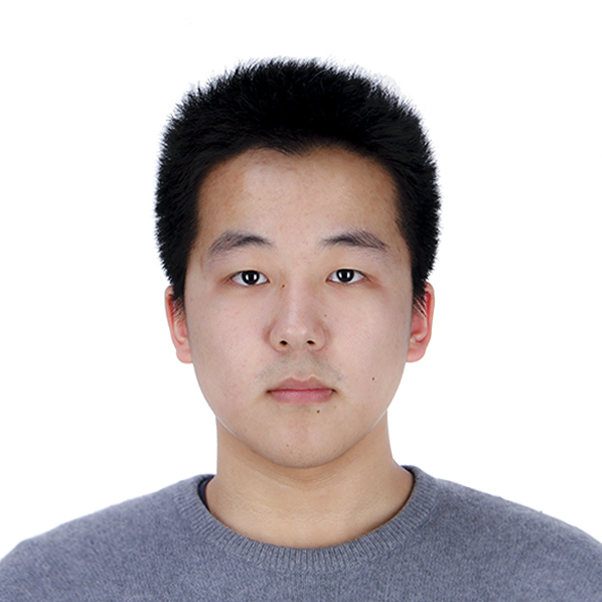
\includegraphics[width=1.5in]{self}
\end{center}

\name{田倍闻}

\basicInfo{
  \email{tianbeiwen88@gmail.com} \textperiodcentered\
  \phone{(+86) 18810033886} \textperiodcentered\
  \github{https://github.com/TB5z035}
}
% \basicInfo{
%   \faBalanceScale \ GPA: 3.85/4 \textperiodcentered\
%   \faUsers \ 年级排名: 30/224 \textperiodcentered\
%   \faLanguage \ 雅思成绩: 7.5/9 \textperiodcentered\
%   \faLanguage \ 英语六级成绩: 612
% }

\section{\faBook\  教育背景}
\datedsubsection{\textbf{清华大学}, 北京}{2018 -- 2019}
\textit{本科}\ 材料科学与工程系
\datedsubsection{\textbf{清华大学}, 北京}{2019 -- 2023}
\textit{本科}\ 计算机科学与技术系
\datedsubsection{\textbf{清华大学}, 北京}{2023至今}
\textit{博士}\ 智能产业研究院,预计 2027 年 6 月毕业

% \section{\faStar\ 课程成绩}
% GPA: 3.85\ /\ 4, 年级排名30\ /\ 224, 部分课程成绩如下:
% \vspace{-0.5em}
% \begin{onehalfspacing}
%   \begin{multicols}{2}
%     \begin{itemize}
%       \item 人工智能导论 \hfill 4.0
%       \item 人工神经网络 \hfill 4.0
%       \item 计算机图形学基础 \hfill 4.0
%       \item 高性能计算导论 \hfill 4.0
%       \item 媒体计算 \hfill 4.0
%       \item 数字逻辑设计 \hfill 4.0
%       \item 编译原理 \hfill 4.0
%       \item 计算机网络原理 \hfill 4.0
%       \item 软件工程 \hfill 4.0
%       \item 以服务为中心的软件开发设计与实现 \hfill 4.0
%     \end{itemize}
%   \end{multicols}
% \end{onehalfspacing}

\section{\faGraduationCap\ 学术成果}


\datedsubsection{\textbf{VIBUS: Data-efficient 3D Scene Parsing with VIewpoint Bottleneck and Uncertainty-Spectrum Modeling}}{}
\role{\textbf{Beiwen Tian}, Liyi Luo, Hao Zhao, Guyue Zhou}{}
\begin{spacing}{1.2}
  \textbf{发表于 ISPRS Journal of Photogrammetry and Remote Sensing (遥感领域期刊 Top1)}
  
  \vspace{0.5em}
  使用数据驱动的深度学习方法对三维场景进行细粒度语义理解,是目前三维视觉的研究重心之一。
  现有工作利用三维场景中点级别的语义标签作为监督信号,以全监督的范式训练逐点输出的神经网络,获得了较好的性能。
  然而,在产业应用场景中,对一个包含数十万点的三维场景进行点级别的语义标注需要大量的人力物力投入,训练数据难以自动化、规模化获取。
  
  \vspace{0.5em}
  本篇工作提出了一种弱监督训练流程,先使用特殊设计的自监督训练范式在大规模无标注三维场景数据上进行表征学习,优化表征空间结构;
  然后将预训练的模型在极少的监督(每场景20-200个标注点)下进行一次微调得到场景中所有点的伪标签;
  最后根据这些伪标签的不确定性和伪标注点与真实标注点在谱空间中的距离,对伪标签的可信度进行建模并用于筛选,得到一套可靠的伪标签并对模型重新训练。
  实验结果显示,本方法在20-200个点的极弱监督信号下,也能实现接近全监督训练情形下的模型性能。
  \textbf{本方法有效解决了三维场景细粒度标注难以高效获取的痛点,建立了一套利用极少数手动标注进行有效训练的方法,大幅节省了数据采集过程需要的资源。}

  \vspace{0.5em}
  \textbf{\underline{本方法在 ScanNet Data Efficient 比赛中获得了弱监督语义分割赛道的冠军\faTrophy}}

  % \vspace{0.5em}
  % 我在本篇工作中做出的贡献是:
  % \begin{itemize}
  %   \item 提出并建立了不确定性—谱空间距离的高维场模型
  %   \item 推导根据不确定性与谱空间距离分布自动选取阈值的EM算法
  %   \item 实现本文提出的方法
  %   \item 设计实验框架,运行大部分实验
  %   \item 将项目方法打包为完整的“手工标注—生成伪标签—筛选可信标签—手动标注”的迭代式工具链,用于AIR-安克项目的交付
  % \end{itemize}  
\end{spacing}

\datedsubsection{\textbf{Unsupervised Road Anomaly Detection with Language Anchors}}{}
\role{\textbf{Beiwen Tian}, Mingdao Liu, Huan-ang Gao, Pengfei Li, Hao Zhao, Guyue Zhou}{}
\begin{spacing}{1.2}
  \textbf{发表于 ICRA 2023}

  \vspace{0.5em}
  在当前的自动驾驶场景中,场景理解模型通常在封集上训练并测试,因而道路异常检测是自动驾驶安全性的重要保障;
  然而收集带有异常语义标注的大规模数据集十分困难。

  \vspace{0.5em}
  因此,本篇工作面向无监督的异常检测,仅使用现有的场景理解模型,利用从大规模多模态模型的语言锚点,分割出异常区域。
  由于这些语言锚点包含丰富的开放集语义信息,该方法在额外训练数据情况下,比以前的无监督方法表现得更好。
  实验表明该方法在多个公开测试集上取得了最高的性能。
  \textbf{本方法首次将大模型引入到道路异常检测任务中,并取得了优越性能。}
\end{spacing}

\datedsubsection{\textbf{From Semi-supervised to Omni-supervised Room Layout Estimation Using Point Clouds}}{}
\role{Huan-ang Gao, \textbf{Beiwen Tian}, Pengfei Li, Xiaoxue Chen, Hao Zhao, Guyue Zhou, Yurong Chen, Hongbin Zha}{}
\begin{spacing}{1.2}
  \textbf{发表于 ICRA 2023}

  \vspace{0.5em}
  房间布局估计是一项重要的机器人视觉任务,能够应用于机器人环境感知和运动规划等任务中。
  常用方法使用点云进行布局估计,但由于标注困难、数据稀缺,性能难以满足应用要求。
  
  \vspace{0.5em}
  本篇工作基于模型的指数移动平均(EMA)思想来处理半监督条件下的房间布局估计任务。
  本篇工作首先定义了一套四元组匹配策略,并基于为布局四元组量身定制的测试指标定义了数项一致性损失;
  此外,提出了一个新的在线伪标签收集算法,将四元组与点云之间的混合距离测量的分布分解为两个组成部分,从而使得伪标签筛选不需要手动选择阈值。
  
  \vspace{0.5em}
  实验结果显示,本篇工作设计的算法在半监督场景下的ScanNet基准测试中达到了最高性能。
  另外,本篇工作还将半监督设置推进到全方位监督设置, 在新标注的ARKitScenes测试集上展示了显著提高的性能。
  \textbf{本方法充分挖掘了大量难以标注的无监督数据中包含的信息,并用于室内场景布局估计,为垂直领域的无监督数据的充分利用提供了新的思路。}
\end{spacing}

\datedsubsection{\textbf{DQS3D: Densely-matched Quantization-aware Semi-supervised 3D Detection}}{}
\role{Huan-ang Gao, \textbf{Beiwen Tian}, Pengfei Li, Hao Zhao, Guyue Zhou}{}
\begin{spacing}{1.2}
  \textbf{发表于 ICCV 2023}
  
  \vspace{0.5em}
  半监督三维物体检测对于难以标注的复杂三维室内场景理解算法至关重要。
  考虑到半监督学习取得的显著进展,本篇工作采用了自学习的框架,并提出了第一个端到端且以密集标注训练的半监督三维物体检测算法。
  为了解决点到体素离散化引起的量化误差,本篇工作推导并实施了实时补偿该量化误差的闭式规则。
  
  \vspace{0.5em}
  实验表明,相比现有方法,本方法在半监督场景的三维物体检测任务上性能大幅领先现有方法。
  \textbf{本方法充分挖掘了大量难以标注的无监督数据中包含的信息,用于三维物体目标检测,并推动半监督学习方式在三维视觉领域的利用。}
\end{spacing}

\datedsubsection{\textbf{Delving into Shape-aware Zero-shot Semantic Segmentation}}{}
\role{Xinyu Liu, \textbf{Beiwen Tian}, Zhen Wang, Rui Wang, Kehua Sheng, Bo Zhang, Hao Zhao, Guyue Zhou}{}
\begin{spacing}{1.2}
  \textbf{发表于 CVPR 2023}
  
  \vspace{0.5em}
  随着大规模多模态预训练模型的迅猛发展,最新的识别模型能够以开集方式分类任意物体,并获得极高准确率。
  然而在语义分割领域难以达到类似的性能,因为精细的形状刻画是语义分割任务的一大重点,而现有的多模态模型使用图像级别的语言描述进行训练。
  
  \vspace{0.5em}
  为了弥补这一差距,本篇工作追求形状引导的开集语义分割,提议利用用自监督像素级特征构建的拉普拉斯矩阵促进形状感知,并深入探讨了在使用不同的主干网络上的不同数据集上实现的性能增益。
  得出结论:对形状的感知程度和语言描述的局部性高度相关。
  
  \vspace{0.5em}
  实验表明,我们的方法在多个数据集的开机语义分割任务上都取得了最高的性能。
  \textbf{本篇工作为多模态预训练模型在语义分割任务上落地应用提供了新的思路。}
\end{spacing}


\datedsubsection{\textbf{TOIST: Task Oriented Instance Segmentation Transformer with Noun-Pronoun Distillation}}{}
\role{Pengfei Li, \textbf{Beiwen Tian}, Yongliang Shi, Xiaoxue Chen, Hao Zhao, Guyue Zhou, Ya-Qin Zhang}{}
\begin{spacing}{1.2}
  \textbf{发表于 NeurIPS 2022}
  
  \vspace{0.5em}
  目前,基于名词理解的算法能够显著提升计算机视觉领域中物体检测以及物体分割的性能;
  然而动词在物体分割任务中的潜在作用目前尚未得到充分探索,动词的高层次语义与物体的可供性的关联在现有的模型中也尚未得到利用。
  
  \vspace{0.5em}
  本篇工作旨在提升基于可供性的物体分割效果;该任务接受行为描述作为输入,要求算法分割出能够完成该行为(具有可供性)的物体。
  本方法基于Transformer架构,设计了名词—代词蒸馏框架以利用现有的名词指代理解模型,将名词蕴含的语义合理推导至动词中,从而在推导过程中获取可供性信息。
  \textbf{本方法首次提出了从名词向代词进行知识蒸馏的训练范式,为图像中动词理解提供了全新视角。}

  % \vspace{0.5em}
  % 我在本篇工作中做出的贡献是:
  % \begin{itemize}
  %   \item 基于Transformer架构实现本文提出的方法
  %   \item 设计实验框架,运行试验
  % \end{itemize}  
\end{spacing}

\datedsubsection{\textbf{Language-guided 3D Semantic Style Transfer of 3D Indoor Scenes}}{}
\role{Bu Jin, \textbf{Beiwen Tian}, Hao Zhao, Guyue Zhou}{}
\begin{spacing}{1.2}
  \textbf{发表于 ACMMM 2022 Workshop PIES-ME}

  \vspace{0.5em}
  在虚拟现实、元宇宙的发展契机下,三维场景的风格迁移成为学界和业界的共同关注点;然而用于风格迁移的监督用真实场景具有多方面问题:1. 采集较为困难,难以规模化;2. 真实场景限于环境条件,难以包含虚拟化或艺术化的场景风格。
  
  \vspace{0.5em}
  本篇工作设计了一个跨模态的优化方法对风格迁移网络进行训练,避免了风格迁移训练数据缺失的问题。
  本方法接受自然语言形式的文本描述以及待迁移的三维场景作为输入,后者经过风格迁移网络以及可微渲染器后的图像输出和文本描述同时经过大规模多模态预训练模型CLIP,在该模型的表征空间中获取二者语义差距以优化风格迁移网络。
  
  \vspace{0.5em}
  该优化过程是逐类完成的,类别标签来自于上一工作生成的伪标签;本方法利用不同类别的语义信息,获得更加精细化的风格迁移效果。为了保证迁移前后的一致性,相同语义区域在HSV空间中的色彩差距也在优化过程中作为额外的监督信号。
  \textbf{本篇工作提出了一种新的三维场景风格迁移方法,能够有效复用现有的高性能多模态预训练模型,依托语义分割网络进行精细化的迁移效果;同时接受自然语言作为输入,摆脱对风格监督数据的依赖。}

  % \vspace{0.5em}
  % 我在本篇工作中做出的贡献是:
  % \begin{itemize}
  %   \item 参与实现本文提出的方法
  %   \item 设计实验框架,运行实验
  %   \item 提出了HSV空间中色彩差距的约束项
  %   \item 开发实现在线用户试验工具平台
  % \end{itemize}  
\end{spacing}



\datedsubsection{\textbf{Unsupervised Cross-Task Generalization via Retrieval Augmentation}}{}
\role{Bill Yuchen Lin, Kangmin Tan, Chris Scott Miller, \textbf{Beiwen Tian}, Xiang Ren}{}
\begin{spacing}{1.2}
  \textbf{发表于 NeurIPS 2022 \& ACL 2022 Workshop LNLS}
  
  \vspace{0.5em}
  大规模自然语言模型在多个任务上的泛化性能,成为目前自然语言处理领域关注的焦点之一。
  大量工作致力于通过优化的模型结构或训练策略,使得预训练语言模型经过极少新任务数据样本(弱监督)的微调,其性能接近在新任务上全监督训练后的表现。
  然而,现有的工作忽视了上游预训练数据对泛化性能产生的潜在影响。
  
  \vspace{0.5em}
  本篇工作旨在在海量上游数据中挖掘更有利于新任务的子集,将预训练模型在该数据子集上进行增强训练后再在新任务的少量样本上微调,以期提高模型在新任务上的性能。
  实验结果显示,进行过增强训练的模型与未增强训练时相比,其在新任务上的性能有显著提升。
  \textbf{本方法有效解决了大规模预训练模型难以高效迁移到下游任务的问题,提高了上游预训练数据的利用率,节省了迁移学习过程的训练时间。}
  
  % \vspace{0.5em}
  % 我在本篇工作中做出的贡献是:
  % \begin{itemize}
  %   \item 进行实验并获取不进行增强的基线模型经微调后在新任务上的表现
  %   \item 参与可行性验证,从上游训练数据中随机取子集对基线模型进行重训练,在不同的子集上获取了强于基线和弱于基线的性能,验证了方法的可行性
  % \end{itemize}  
\end{spacing}


\section{\faServer\ 科研项目}
\datedsubsection{\textbf{AIR-百度自动驾驶白皮书2.0的科学原理验证和报告撰写}}{2022年3月}

我在Carla仿真环境中设计实验,\textbf{验证了车路协同时对异常物体的检测效果优于单车感知时的性能};另外,我也\textbf{参与撰写了白皮书附录部分关于异常物体分割模型的相关内容。}

\datedsubsection{\textbf{弱监督半自动点云标注训练框架}}{2022年4月}
\role{AIR-安克项目交付成果之一}{}
我实现了对三维点云进行“手工标注—生成伪标签—筛选可信标签—手动标注”的迭代式工具链,能够基于手动标注的极少数标签,迭代地生成大量可信伪标签,用作深度学习模型的训练与优化。
\textbf{该工具能够减少对大规模点云(数十万个点)进行手工点级别标注所需要的大量人力物力资源,打通了数据采集-训练的闭环,加速数据落盘。}



\section{\faCogs\ 实习经历}
\datedsubsection{\textbf{智能产业研究院}, 清华大学}{2021 年 9 月 -- 至今}
\role{GPU集群搭建与维护}{}
自 2021 年 9 月至今,\textbf{我负责AIR所有公用GPU服务器的环境搭建和日常维护}。在此期间完成了:
\begin{itemize}[parsep=0.5ex]
  \item 设计\textbf{统一入口—分布计算—统一存储}的集群架构
  \item 实现运算节点虚拟化,管理私有虚拟化云平台
  \item 搭建共计6台物理机12个运算节点的基础运行环境
  \item 搭建\textbf{全局任务队列}“Slurm”,将统一入口提交到任务自动化分发到运算节点上执行
  \item 解决偶发集群服务器宕机、无响应、内存耗尽、存储空间耗尽等问题
\end{itemize}
\vspace{0.5em}
\role{AIR DISCOVER 实验室网站搭建}{}
我搭建了AIR DISCOVER实验室的网站,搭建了内容框架,并以三维模型的方式的方式呈现了实验室布局。
网站首页:\href{https://www.discover-lab.com}{https://www.discover-lab.com}

\datedsubsection{\textbf{计算机科学与技术系}, 清华大学}{2020 年9月 -- 至今}
\role{《软件工程》课程助教}{}
% increase linespacing [parsep=0.5ex]

\section{\faChild \ 社工与志愿经历}
\datedsubsection{\textbf{清华大学计86班班长}}{2020 年 9月 -- 2021年9月}
\vspace{0.5em}
\datedsubsection{\textbf{清华大学“答疑坊”特级志愿者}}{2020 年8月 至今}
志愿时长144小时


\section{\faTrophy\ 获奖情况}
\datedline{\textbf{清华之友-黄奕聪伉俪奖助学金}, 学业优秀奖学金}{2021 年 10 月}
\vspace{0.5em}
\datedline{\textbf{志愿优秀奖学金}}{2021 年 10 月}
\vspace{0.5em}
\datedline{\textbf{SUMMER AIR 2021夏令营}, 第一名}{2021 年8 月}
\role{项目}{弱监督条件下的三维场景语义分割}
\vspace{0.5em}

% \section{\faInfo\ 其他}
% increase linespacing [parsep=0.5ex]

%% Reference
%\newpage
%\bibliographystyle{IEEETran}
%\bibliography{mycite}
\end{document}
